\documentclass[11pt,a4paper]{article}
\usepackage[utf8]{inputenc}
\usepackage[T1]{fontenc}
\IfFileExists{lmodern.sty}{\usepackage{lmodern}}{}
\usepackage[margin=2.3cm]{geometry}
\usepackage{amsmath,amssymb}
\usepackage{graphicx}
\usepackage{booktabs}
\usepackage{xcolor}
\usepackage{caption}
\usepackage{fancyhdr}
\usepackage[colorlinks=true,linkcolor=blue!50!black,citecolor=blue!50!black,urlcolor=blue!50!black]{hyperref}

\pagestyle{fancy}
\fancyhf{}
\fancyhead[L]{O. Zaidi --- CRNA}
\fancyhead[R]{Final report (draft)}
\fancyfoot[C]{\thepage}

% Placeholder for material still to be produced or checked
\newcommand{\todo}[1]{\par\smallskip\noindent\fcolorbox{orange!70!black}{orange!8}{\parbox{\dimexpr\linewidth-2\fboxsep-2\fboxrule}{\small\textbf{To complete:} #1}}\par\smallskip}
\newcommand{\NH}{NH$_3$}
\newcommand{\CH}{CH$_4$}
\newcommand{\aone}{3a$_1$}
\newcommand{\atwo}{2a$_1$}

\title{\textbf{Application of the three-Coulomb-wave model with variable charge (3CWZ)\\
to the single ionization of CH$_4$ and NH$_3$ by electron impact}\\[4pt]
\large Final report of the research protocol --- \textcolor{orange!70!black}{DRAFT}}
\author{Omar Zaidi\\ Division de Physique, Centre de Recherche Nucl\'eaire d'Alger\\
Supervision: N. Zenine}
\date{2026}

\begin{document}
\maketitle
\thispagestyle{fancy}

\begin{abstract}
We extend the three-Coulomb-wave model with a position-dependent effective charge (3CWZ) from
atomic to molecular targets and apply it to the single ionization of \CH{} and \NH{} by electron
impact.
\begin{itemize}
\item \textbf{Target:} described by the one-centre SCF molecular orbitals of Moccia. The random
  orientation of the molecule is averaged analytically.
\item \textbf{Effective charges:} derived from the monopole part of the Hartree potential of the SCF
  density, with a self-interaction correction for the ejected electron.
\item \textbf{Code:} we implemented the model in a parallel Fortran code. We validated it against
  the original \CH{} code and against analytic limits.
\item \textbf{Comparisons for \NH{}:}
  \begin{itemize}
  \item triple differential cross sections measured by El~Mir \emph{et al.} at $E_s=500$~eV,
    $\theta_s=-6^\circ$, $E_e=74$~eV;
  \item electron momentum spectroscopy profiles (1200~eV);
  \item double differential cross sections at $E_i=500$~eV.
  \end{itemize}
\end{itemize}
The binary peak is well reproduced for the three valence orbitals \aone, 1e and \atwo. The recoil
peak is underestimated by a factor 5--10. We trace this deficit to the ejected-electron wave: the
variable-charge Coulomb wave does not solve the one-electron equation in the screened ionic
potential, and it misses the strong back-scattering by the NH$_3^+$ core. We delimit the
kinematic and numerical domain of validity of the model, and we propose a distorted-wave treatment
of the ejected electron as the next step.
\todo{Update the abstract with the \CH{} results, the PCI study and the variable- versus
constant-charge comparison (Sections~\ref{sec:ch4}--\ref{sec:zconst}).}
\end{abstract}

\tableofcontents
\newpage

%=====================================================================
\section{Introduction}
%=====================================================================
Electron-impact ionization is a basic process in collision physics. It is also a key input for:
\begin{itemize}
\item plasma modelling;
\item atmospheric and astrophysical chemistry;
\item radiation--matter interaction, where low-energy secondary electrons produced by ionizing
  radiation cause further ionization and fragmentation of biomolecules.
\end{itemize}
Kinematically complete $(e,2e)$ experiments measure the triple differential cross section (TDCS).
The TDCS is sensitive both to the structure of the target and to the dynamics of the three
charged particles in the final state.

Theoretical descriptions form a hierarchy of approximations:
\begin{itemize}
\item the plane-wave Born approximation (PWBA);
\item distorted-wave methods (DWBA, M3DW);
\item three-Coulomb-wave models (3C or BBK)~\cite{Brauner1989}, which treat the three two-body
  Coulomb interactions of the final state on an equal footing.
\end{itemize}
The 3CWZ model~\cite{Bechane2024,Tamin2024,Zaidi2024} replaces the constant charges of the 3C
model by a position-dependent effective charge $Z(r)$. This charge interpolates between the
nuclear charge near the nucleus and the ionic charge far from it. It has improved the description
of atomic targets.

Molecules add several difficulties:
\begin{itemize}
\item the potential is multi-centre and non-spherical;
\item the orientation of the molecule is random;
\item the orbital structure is more complex.
\end{itemize}
\CH{} and \NH{} are ten-electron hydrides whose C--H and N--H bonds are building blocks of
biological molecules. \CH{} is nearly spherical. \NH{} is more anisotropic and has a permanent
dipole moment.

The objectives of the protocol were:
\begin{itemize}
\item[O1.] adapt the 3CWZ formalism to molecular targets with the one-centre orbitals of Moccia,
  including $Z(r)$ for each orbital;
\item[O2.] compute TDCS for the orbitals of \CH{} and \NH{} under various kinematics;
\item[O3.] study the post-collision interaction (PCI) by comparing results with and without the
  electron--electron factor $C_{ab}$;
\item[O4.] validate the model against the available experimental and theoretical data.
\end{itemize}
The expected outcomes were to show what the variable charge contributes and to delimit the domain
of validity of the model for molecules.

The report is organised as follows:
\begin{itemize}
\item Section~\ref{sec:theory}: the formalism;
\item Section~\ref{sec:numerics}: the numerical implementation and its validation;
\item Section~\ref{sec:results}: the results;
\item Section~\ref{sec:discussion}: the origin of the recoil-peak deficit and the domain of validity;
\item Section~\ref{sec:conclusion}: conclusions and perspectives.
\end{itemize}
Atomic units are used throughout unless stated otherwise.

%=====================================================================
\section{Theory}\label{sec:theory}
%=====================================================================
\subsection{Kinematics and cross section}
We consider $e^-(\mathbf k_i)+M\to M^++e^-(\mathbf k_s)+e^-(\mathbf k_e)$, with
\begin{equation}
E_i=E_s+E_e+I_n,\qquad \mathbf K=\mathbf k_i-\mathbf k_s,\qquad \mathbf q=\mathbf K-\mathbf k_e ,
\end{equation}
where:
\begin{itemize}
\item $I_n$ is the binding energy of the ionized orbital;
\item $\mathbf K$ is the momentum transfer;
\item $\mathbf q$ is the recoil momentum of the ion.
\end{itemize}
The TDCS is
\begin{equation}
\sigma^{(3)}=\frac{d^3\sigma}{d\Omega_s\,d\Omega_e\,dE_e}=(2\pi)^4\frac{k_sk_e}{k_i}\,|T_{fi}|^2 .
\end{equation}
At the energies considered here ($E_s\gg E_e$), exchange is neglected and $T_{fi}=T_{dir}$.
\todo{If the low-energy data of Nixon \emph{et al.}~\cite{Nixon2013} are analysed, include the
exchange amplitude. Check the factor $\tfrac12$ of the spin average:
$\tfrac12\left(|T_d|^2+|T_e|^2+|T_d-T_e|^2\right)$.}

\subsection{The 3CWZ final state}
The final state is the product of three Coulomb waves:
\begin{equation}
\Psi_f=\phi^-_s(\mathbf k_s,\mathbf r_0)\,\phi^-_e(\mathbf k_e,\mathbf r_1)\,C^-_{se}(\mathbf k_{se},\mathbf r_{01}),
\qquad \mathbf k_{se}=\tfrac12(\mathbf k_s-\mathbf k_e),
\end{equation}
Each electron--ion wave has the form
\begin{equation}
\phi^{\pm}_c(\mathbf k,\mathbf r)=(2\pi)^{-3/2}\,e^{\pi\alpha(r)/2}\,\Gamma\!\left(1\mp i\alpha(r)\right)
e^{i\mathbf k\cdot\mathbf r}\,{}_1F_1\!\left(\pm i\alpha(r);1;\pm i(kr\mp\mathbf k\cdot\mathbf r)\right),
\qquad \alpha(r)=\frac{Z(r)}{k}.
\label{eq:cwz}
\end{equation}
\begin{itemize}
\item The effective charge $Z(r)$ goes to 1 at large $r$ for the scattered and ejected electrons,
  and to 0 for the incident electron (neutral target).
\item The incident wave $\phi^+_i(\mathbf k_i,\mathbf r_0)$ uses the neutral-target charge.
\item The factor $C_{se}$ describes the electron--electron interaction (PCI), with
  $\alpha_{se}=-1/(2k_{se})$.
\end{itemize}

In the frozen-core, one-active-electron approximation the interaction is
$V=-1/r_0+1/r_{01}$, and the direct amplitude is
\begin{equation}
T_{dir}=\Big\langle\Psi_f\Big|\frac1{r_{01}}-\frac1{r_0}\Big|\phi^+_i\,\Phi\Big\rangle=T^1-T^0 .
\end{equation}
\begin{itemize}
\item The six-dimensional integrals are made separable by a Fourier representation of $C_{se}$.
\item Each wave is split into a $Z=1$ (or $Z=0$) Coulomb part, which is integrated analytically,
  and a short-range correction confined to $r<d$, which is integrated numerically.
\item The cut-off is $d=4$ a.u. It is justified by $Z_{ion}(4)=1.011$ (Section~\ref{sec:zr}).
\end{itemize}
The full derivation is given in the 2nd-quarter report.

\subsection{Molecular target and orientation average}
The molecular orbitals are the one-centre SCF orbitals of Moccia~\cite{Moccia1964a,Moccia1964b}.
They are expanded on Slater functions centred on the heavy atom:
\begin{equation}
\Phi(\mathbf r)=\sum_j c_j\,\frac{(2\zeta_j)^{n_j+1/2}}{\sqrt{(2n_j)!}}\,r^{n_j-1}e^{-\zeta_jr}\,S_{l_jm_j}(\hat{\mathbf r}),
\end{equation}
where $S_{lm}$ are real spherical harmonics. For \NH{} we use Table~I of Moccia~II: pyramidal
geometry, $R_{\rm N-H}=1.928$ a.u., $\theta=108.9^\circ$, with the valence orbitals \atwo, 1e and
\aone{} (vertical ionization energies 27.0, 16.4 and 10.85 eV).

The amplitude is linear in the orbital. Each orbital is therefore split into parts $g$ of given
$(l_g,m_g)$, $\Phi=\sum_gR_g(r)S_{l_gm_g}$. The orthogonality of the rotation matrices,
\begin{equation}
\frac1{8\pi^2}\int d\Omega_{\rm Euler}\,D^{l}_{\mu m}D^{l'*}_{\mu'm'}=\frac{\delta_{ll'}\delta_{mm'}\delta_{\mu\mu'}}{2l+1},
\end{equation}
then gives the orientation-averaged TDCS exactly:
\begin{equation}
\langle\sigma^{(3)}\rangle=(2\pi)^4\frac{k_sk_e}{k_i}\sum_g\frac{1}{2l_g+1}\sum_{\mu=-l_g}^{l_g}\big|T[R_gY_{l_g\mu}]\big|^2 .
\end{equation}

\subsection{Variable effective charge}\label{sec:theory-z}
Following the 3rd-quarter report, $Z(r)=r\,V_{\rm total}(r)$, where $V_{\rm total}$ is the
monopole ($L=0$) part of the electrostatic potential of the target. It has three contributions:
\begin{itemize}
\item the heavy nucleus;
\item the Hartree potential of the SCF electron density;
\item the hydrogen nuclei, modelled as a uniform spherical shell of charge $n_H$ at radius $a_H$.
\end{itemize}
For each pair of Slater functions of the same $(l,m)$ part, the screening integral has the
closed form
\begin{equation}
b(r)=\frac{p!}{c^{p+1}}-J_p(c,r)+r\,J_{p-1}(c,r),\qquad
J_n(\alpha,r)=\int_r^\infty t^ne^{-\alpha t}dt ,
\end{equation}
with $p=n_i+n_j$ and $c=\zeta_i+\zeta_j$. Then
\begin{equation}
Z(r)=Z_N-\sum_{\rm MO}n_{\rm MO}\sum_{\rm pairs}c_ic_jN_iN_j\,b(r)+n_H\min(r/a_H,1).
\end{equation}
\begin{itemize}
\item \textbf{Incident electron:} sees the full density, so $Z\to Z_N-N_e+n_H=0$.
\item \textbf{Ejected and scattered electrons:} one electron is removed from the ionized orbital
  (self-interaction correction), so $Z\to1$.
\end{itemize}

%=====================================================================
\section{Numerical implementation and validation}\label{sec:numerics}
%=====================================================================
\subsection{Code}
The code \texttt{nh3\_opt\_claude.for} generalizes the \CH{} 3CWZ code to any XH$_n$ target
described by Slater-type one-centre orbitals. Its main features are:
\begin{itemize}
\item The target data (nuclear charge, proton shell, all occupied orbitals and their $(l,m)$
  parts) are given in one routine. The ionized orbital is selected by a switch.
\item $Z(r)$ is computed from these data for the neutral molecule and for the ion.
\item The $Z=1$ parts of the ejected-electron integrals are analytic. The short-range corrections
  ($r<d$) use Gauss--Legendre quadrature: 4 radial intervals $\times$ 10 points, and $10\times10$
  angular points.
\item The Fourier integral over $\mathbf p$ uses $60\times40\times40$ points, refined around
  $|\mathbf p|=K$.
\item In coplanar geometry, the mirror symmetry $y\to-y$ halves the cost.
\item The code is parallelized with OpenMP. A coplanar angular distribution (61 ejection angles)
  takes about 3~min on 4 cores.
\end{itemize}

\subsection{Validation}
\begin{itemize}
\item With the \CH{} target, the code reproduces the original \CH{} code exactly.
\item Analytic and numerical evaluations of the $Z=1$ ejected-electron integral agree to $10^{-7}$.
\item The mirror-symmetric and full angular grids give identical results.
\item All molecular orbitals are normalised to $1\pm10^{-5}$.
\item $Z(r)$ reaches its asymptotic values 0 (neutral) and 1 (ion).
\end{itemize}

\subsection{Options tested}
\begin{itemize}
\item \texttt{isr=1}: the projectile--core interaction $-1/r_0$ is replaced by the screened static
  potential $-Z_{ion}(r_0)/r_0$, i.e.\ its short-range part is added.
\item \texttt{iorth=1}: the ejected wave is Schmidt-orthogonalized to the ionized orbital, partial
  wave by partial wave, before the amplitude is computed.
\end{itemize}

\subsection{Numerical domain of validity}\label{sec:conv}
We repeated calculations with finer grids: 16 points per interval, 8 radial intervals for the
projectile and 4 for the ejected electron. The default grids are accurate to about 20\% when both
outgoing electrons are slow and the momentum transfer is small ($K\lesssim3$ a.u.). This holds,
for example, for the El~Mir kinematics ($K\approx0.85$~a.u., $E_e=74$~eV). Outside this domain
they are not accurate:
\begin{itemize}
\item for a 600~eV ejected electron (EMS kinematics), the TDCS changes by up to $+70\%$;
\item at large momentum transfer ($\theta_s\gtrsim40^\circ$ at $E_i=500$~eV), the TDCS is
  overestimated by factors up to 30.
\end{itemize}
Integrated cross sections, which sample large $K$, therefore need grids adapted to $K$.
\todo{Implement $K$-adapted grids, or switch to the analytic $Z=1$ limit beyond $K\approx3$ a.u.,
and repeat the convergence study.}

%=====================================================================
\section{Results}\label{sec:results}
%=====================================================================
\subsection{Effective charges}\label{sec:zr}
\begin{figure}[h]\centering
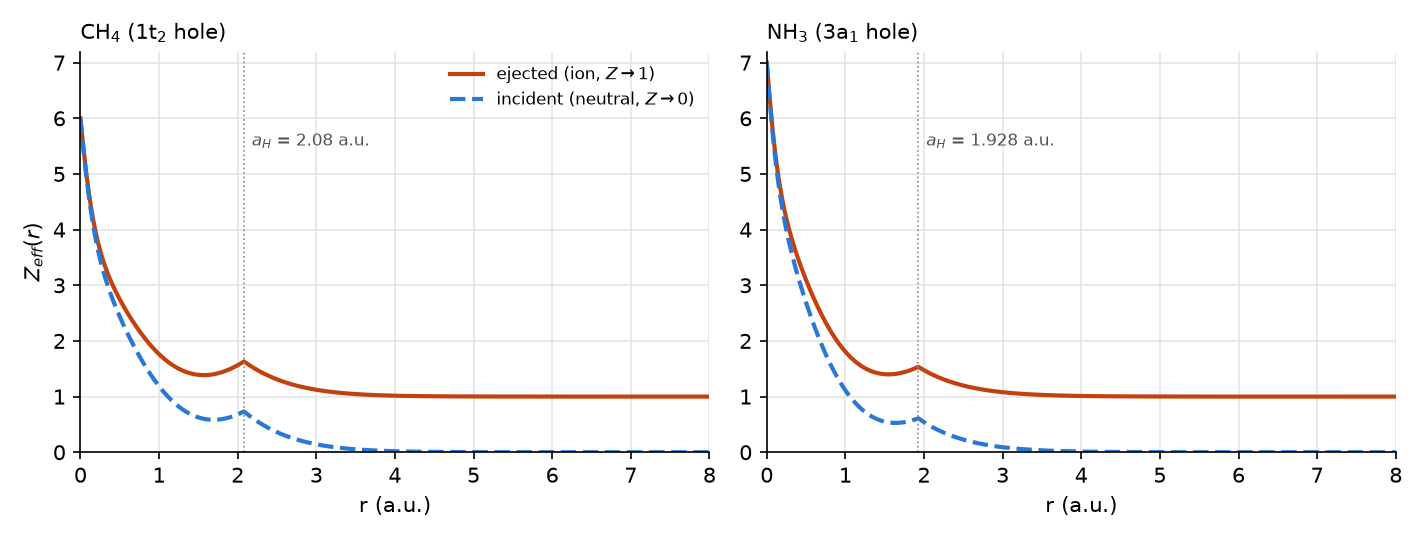
\includegraphics[width=0.92\linewidth]{figs/zr.png}
\caption{Effective charge $Z(r)$ of \CH{} (1t$_2$ hole) and \NH{} (\aone{} hole) for the ejected
electron (ion) and the incident electron (neutral molecule). The dotted line marks the
X--H distance $a_H$.}\label{fig:zr}
\end{figure}

Figure~\ref{fig:zr} and Table~\ref{tab:zr} show the computed charges.
\begin{itemize}
\item Both curves start from $Z_N$: 6 for \CH, 7 for \NH.
\item They fall steeply inside $r\approx1$~a.u.
\item They show a local maximum at the X--H distance, where the proton shell stops contributing.
\item They reach their asymptotes by $r\approx4$~a.u.
\item The ejected-electron charge lies above the incident one at every $r$; this is the
  self-interaction correction.
\item The three \NH{} orbitals give nearly identical $Z_{ion}(r)$ (within 0.05).
\end{itemize}

\begin{table}[h]\centering\small
\caption{$Z(r)$ for \NH{} from the code.}\label{tab:zr}
\begin{tabular}{lcccccccc}\toprule
$r$ (a.u.) & 0 & 0.5 & 1.0 & 1.5 & 2.0 & 2.5 & 3.0 & 4.0\\\midrule
incident (neutral) & 7.000 & 2.690 & 1.113 & 0.549 & 0.541 & 0.227 & 0.091 & 0.013\\
ejected (\aone{} hole) & 7.000 & 3.094 & 1.806 & 1.402 & 1.474 & 1.198 & 1.079 & 1.011\\\bottomrule
\end{tabular}
\end{table}

\subsection{\NH: TDCS in asymmetric coplanar kinematics}
We consider the conditions of El~Mir \emph{et al.}~\cite{ElMir2020}: $E_s=500$~eV, $\theta_s=-6^\circ$,
and $E_e=74$~eV. The incident energy follows from $E_i=E_s+E_e+I_n$. The experimental data were
digitized from the published figures. Being on a relative scale, each calculation is scaled to the
maximum of the experimental binary peak. The momentum transfer points at $\theta_K\approx46$--$50^\circ$.

\begin{figure}[h]\centering
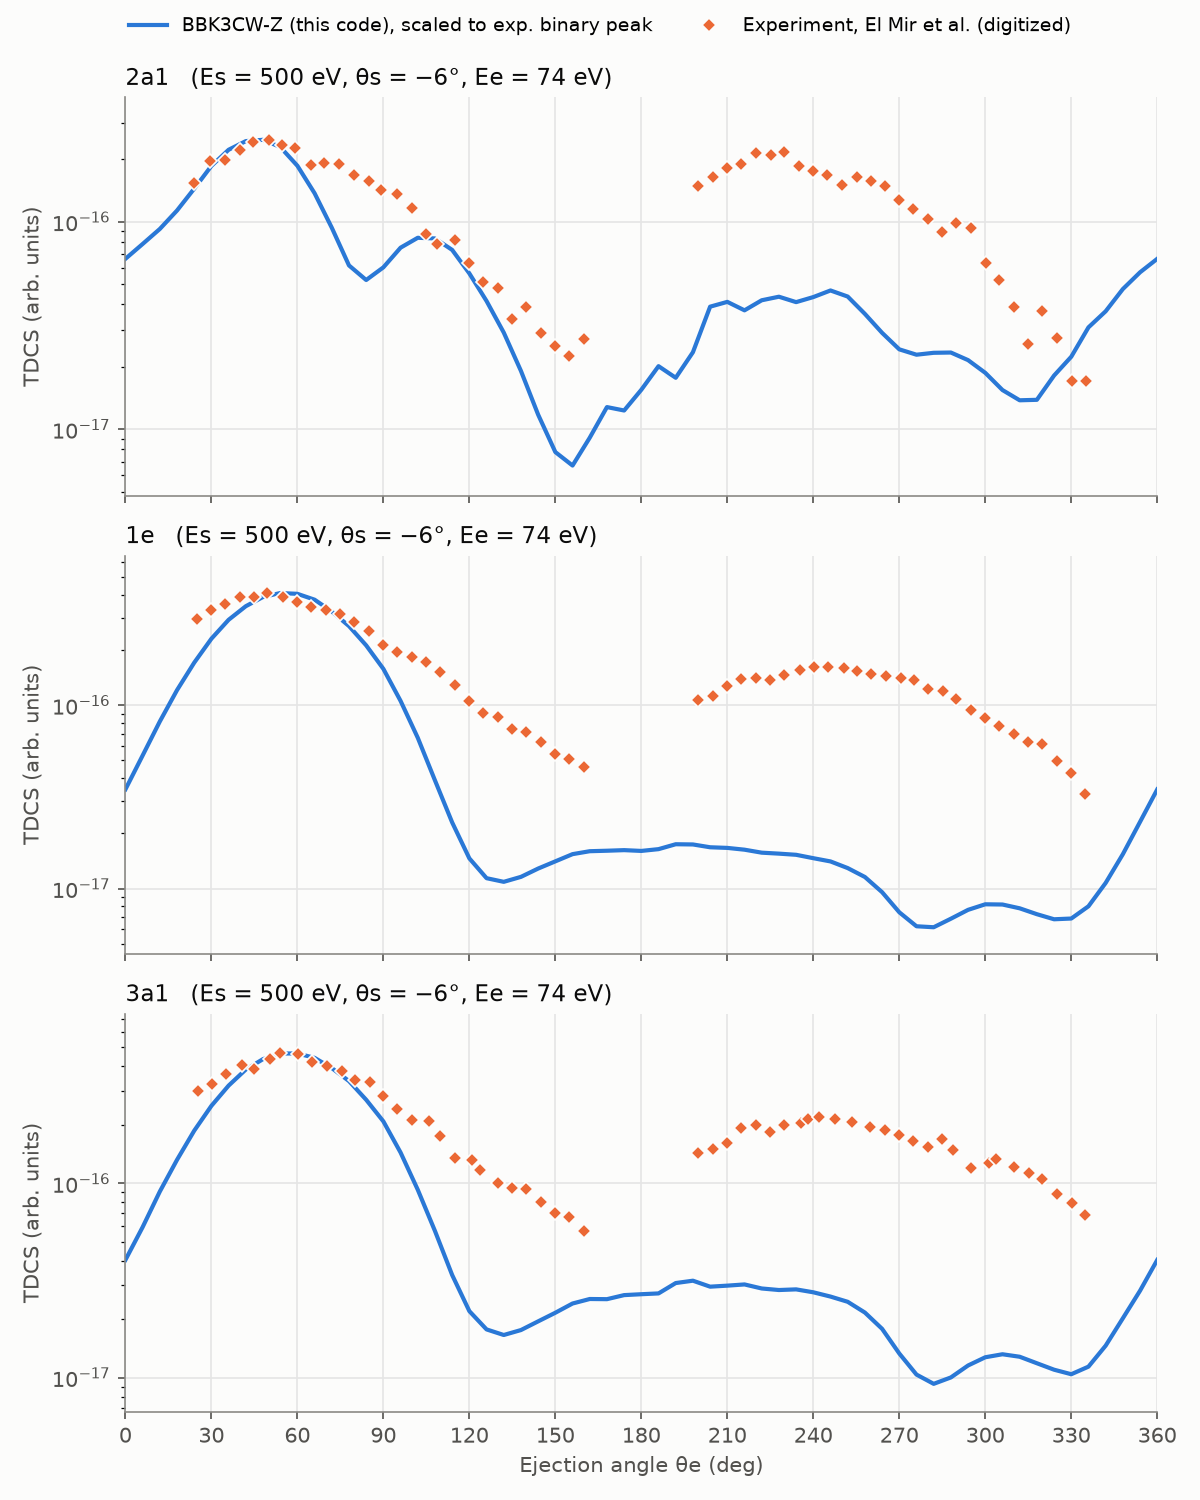
\includegraphics[width=0.66\linewidth]{figs/elmir_base.png}
\caption{TDCS for the \atwo, 1e and \aone{} orbitals of \NH{} at $E_s=500$~eV, $\theta_s=-6^\circ$,
$E_e=74$~eV: 3CWZ (line) and experiment~\cite{ElMir2020} (symbols).}\label{fig:elmir}
\end{figure}

\begin{table}[h]\centering\small
\caption{Peak positions and binary-to-recoil ratios at $E_e=74$~eV.}\label{tab:br}
\begin{tabular}{llccc}\toprule
Orbital & & binary peak & recoil peak & binary/recoil\\\midrule
\aone & experiment & $54^\circ$ & $242^\circ$ & 2.1\\
      & 3CWZ & $60^\circ$ & flat & 14.8\\
1e    & experiment & $49^\circ$ & $240^\circ$ & 2.5\\
      & 3CWZ & $54^\circ$ & flat & 23.4\\
\atwo & experiment & $50^\circ$ & $230^\circ$ & 1.1\\
      & 3CWZ & $48^\circ$ & $246^\circ$ (weak) & 5.3\\\bottomrule
\end{tabular}
\end{table}

Figure~\ref{fig:elmir} and Table~\ref{tab:br} show the following:
\begin{itemize}
\item The position and the front side of the binary peak are reproduced for all three orbitals.
\item The recoil region is underestimated by a factor 5--10. So is the large-angle side of the
  binary peak: at $\theta_e=120^\circ$, the 1e and \aone{} data are about 7 times above the model.
\item For \atwo{} the model shows a dip at about $80^\circ$, the node of the 2s-like momentum
  distribution, which the experiment does not show.
\end{itemize}
\todo{Digitize the $E_e=37$~eV data of~\cite{ElMir2020} and compare with the calculations already
done at that energy.}

\subsection{Short-range projectile potential and orthogonalization}
\begin{figure}[h]\centering
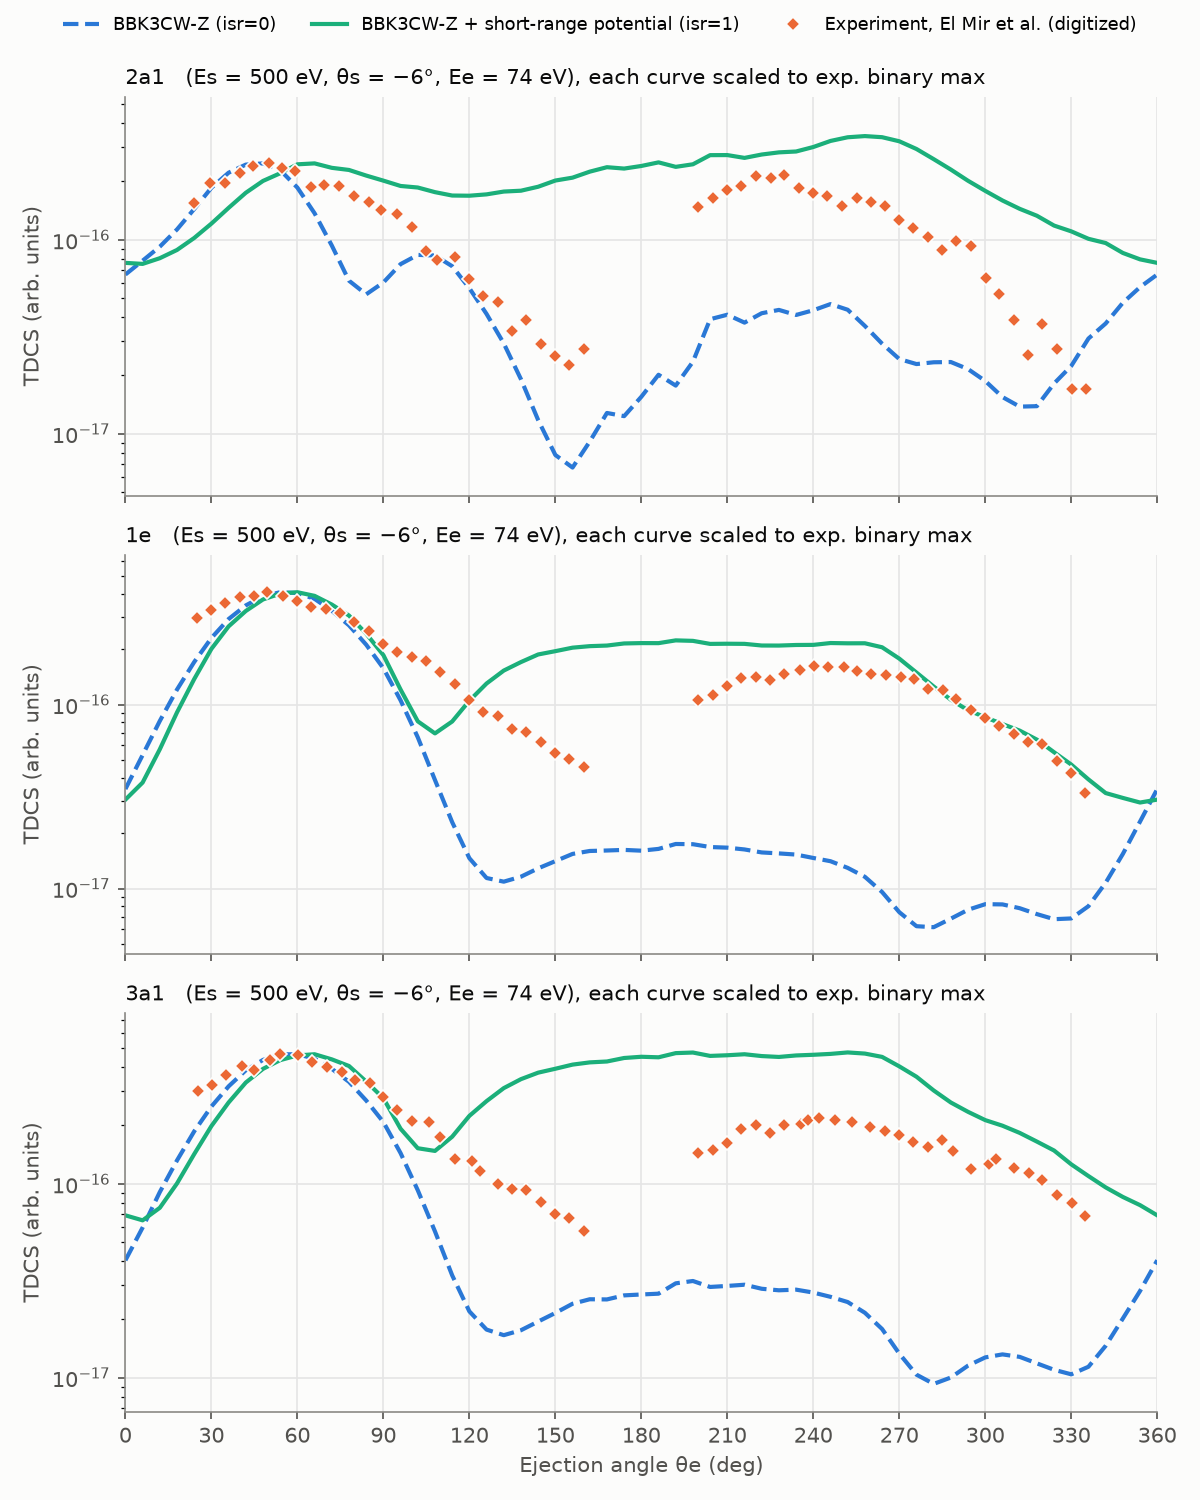
\includegraphics[width=0.49\linewidth]{figs/elmir_sr.png}\hfill
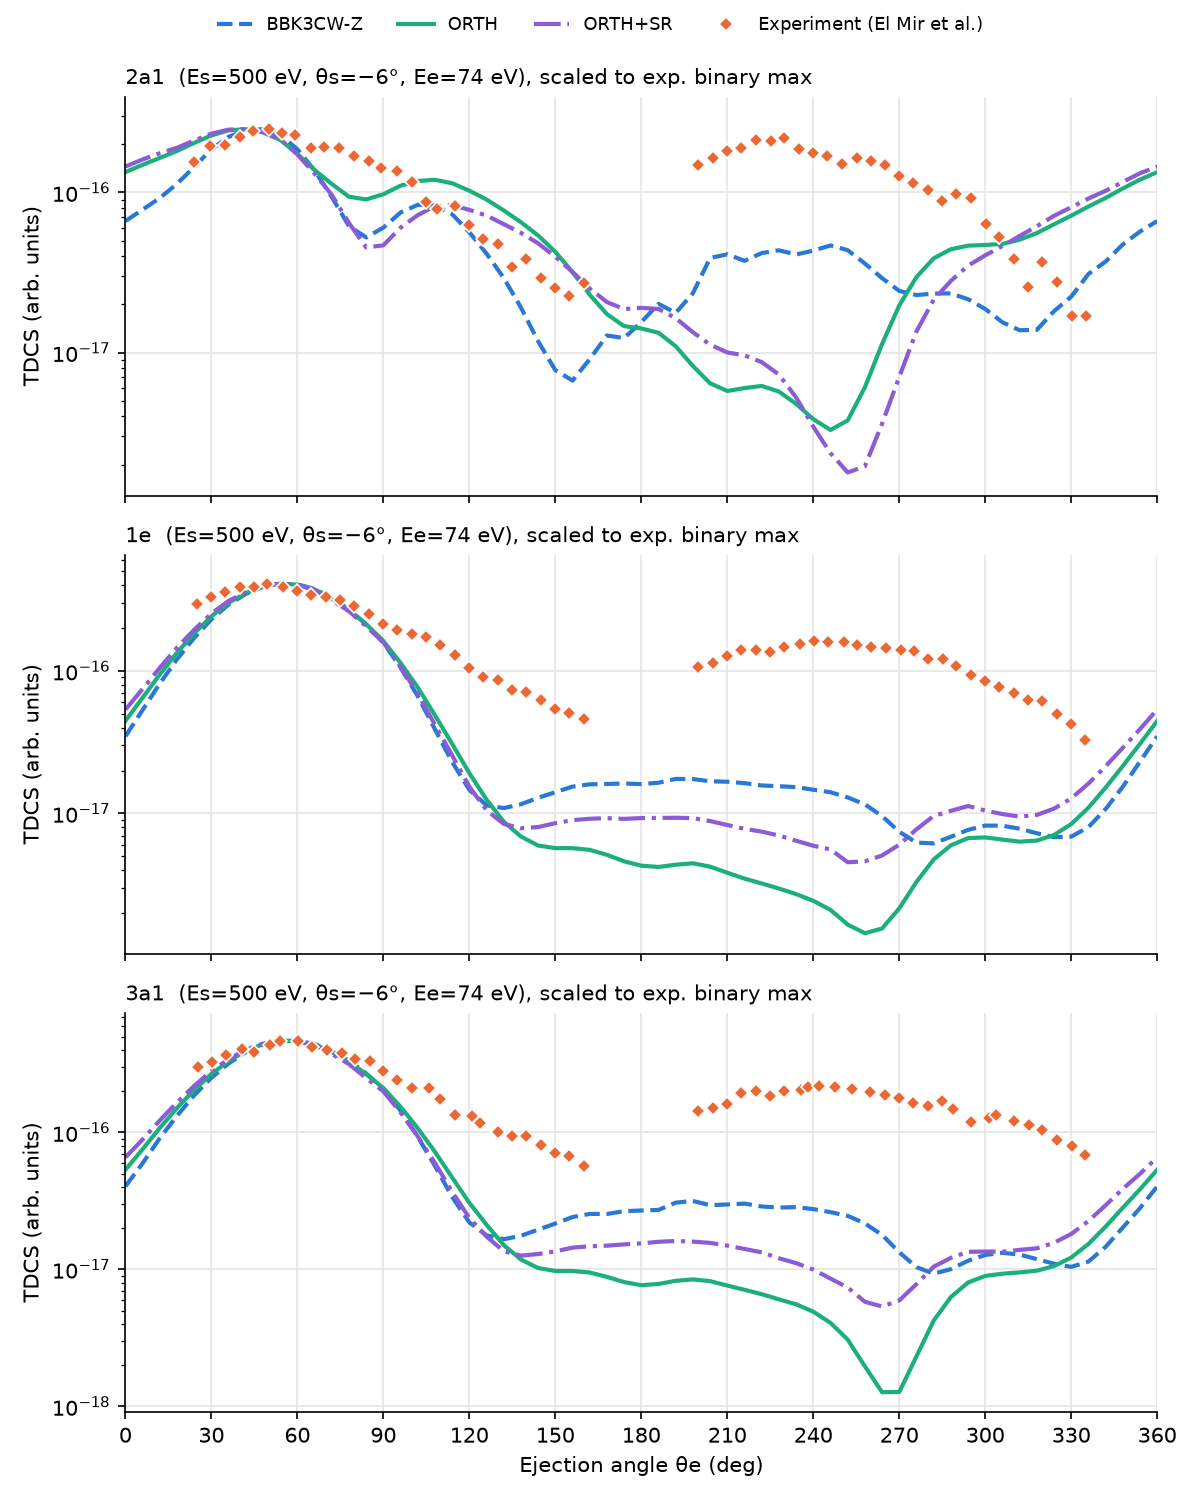
\includegraphics[width=0.49\linewidth]{figs/elmir_orth.png}
\caption{Left: 3CWZ without (dashed) and with (solid) the short-range projectile--core potential.
Right: 3CWZ, orthogonalized ejected wave, and orthogonalized wave with the short-range potential.
Same kinematics as Fig.~\ref{fig:elmir}.}\label{fig:srorth}
\end{figure}

\textbf{Short-range potential (\texttt{isr=1}, Fig.~\ref{fig:srorth}, left).}
\begin{itemize}
\item It raises the cross section at large angles, giving binary/recoil ratios of 0.98, 1.8 and
  0.7 for \aone, 1e and \atwo{}.
\item The rise is nearly isotropic, a shelf rather than a peak centred on $-\mathbf K$.
\item It shifts the binary peak forward to 60--66$^\circ$ and distorts it for \atwo.
\end{itemize}
The ejected Coulomb wave is not orthogonal to the bound orbital. The overlaps are 0.37 for the s
part of \atwo, and 0.10 (s) and 0.18--0.20 (p) for \aone. Through these overlaps the
projectile--core term produces this spurious isotropic contribution.

\textbf{Orthogonalization (\texttt{iorth=1}, Fig.~\ref{fig:srorth}, right).}
\begin{itemize}
\item It removes the shelf, and the \atwo{} binary peak recovers its shape.
\item The recoil region drops back to about 10 times below the data.
\end{itemize}
The physical back-scattering contained in the 3CWZ ejected wave is therefore too weak.

\subsection{\NH: electron momentum spectroscopy}
As a test of the orbitals and of the high-energy limit, we computed the momentum profiles measured
by Bawagan \emph{et al.}~\cite{Bawagan1988}: $E_0=1200$~eV$+I_n$, symmetric non-coplanar geometry,
$\theta=45^\circ$, 600~eV each (Fig.~\ref{fig:ems}).
\begin{itemize}
\item The peak positions are reproduced (q $\approx$ 0.58, 0.1 and 0.57~a.u.), and so are the
  shapes for \atwo{} and \aone.
\item The 1e profile is about 1.5 times low above $q\approx1.3$~a.u. The paper's PWBA shows the
  same, so the cause is the high-momentum content of the 1e orbital.
\item The absolute values with the default grids are 0.57 of the PWBA of Rezkallah
  \emph{et al.}~\cite{Rezkallah2011}. With finer grids, 3a$_1$ reaches 0.76; see Section~\ref{sec:conv}.
\end{itemize}

\begin{figure}[h]\centering
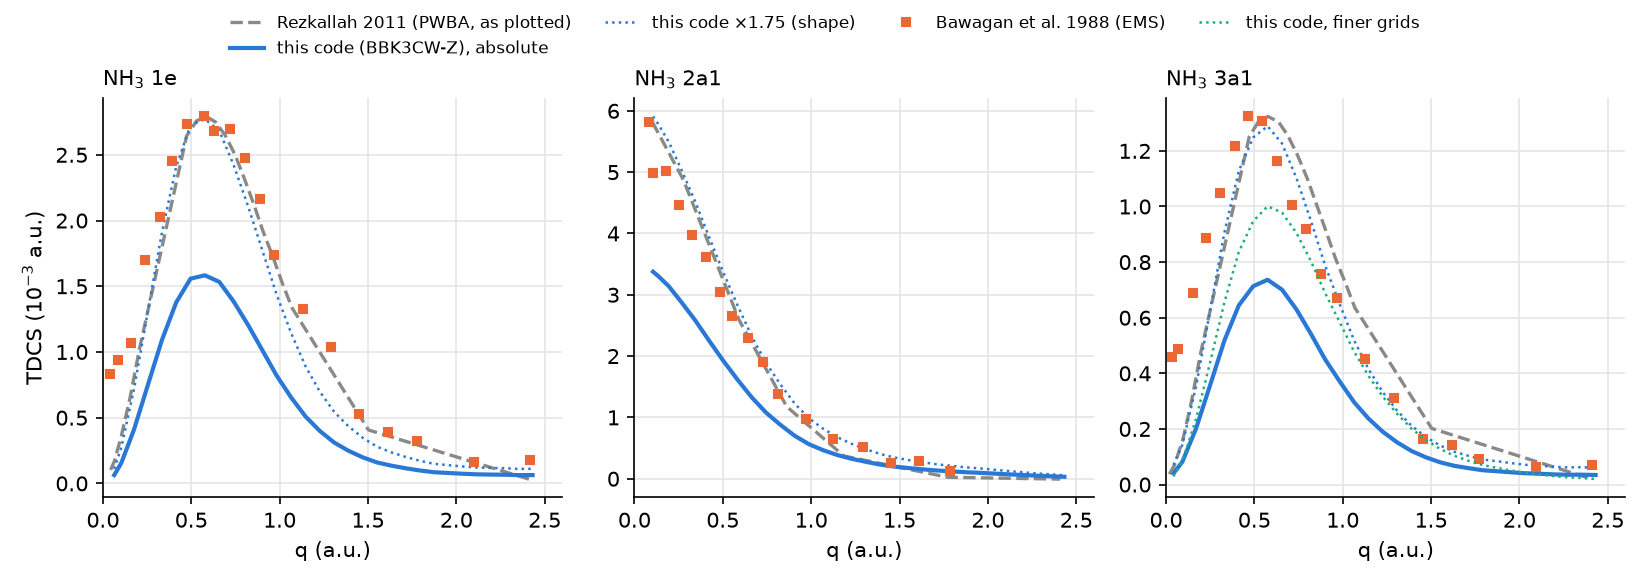
\includegraphics[width=\linewidth]{figs/ems.png}
\caption{\NH{} momentum profiles at 1200 eV: 3CWZ (absolute, and scaled by 1.75), PWBA of
Ref.~\cite{Rezkallah2011}, and experiment~\cite{Bawagan1988}.}\label{fig:ems}
\end{figure}

\subsection{\NH: double differential cross section}
We integrated the TDCS over the scattered-electron direction:
\begin{itemize}
\item 17 points equally spaced in $\ln K$ and 5 azimuths;
\item the three valence orbitals summed, with 1e counted twice.
\end{itemize}
This gives the DDCS at $E_i=500$~eV and $\theta_e=120^\circ$ (Fig.~\ref{fig:ddcs}). The model
exceeds the data of Opal \emph{et al.}~\cite{Opal1972} by factors of 1.79, 1.58 and 1.35 at
$E_e=5$, 20 and 60~eV. At 150~eV the excess (factor 7) comes from large momentum transfers, where
the default grids are not converged (Section~\ref{sec:conv}).

\begin{figure}[h]\centering
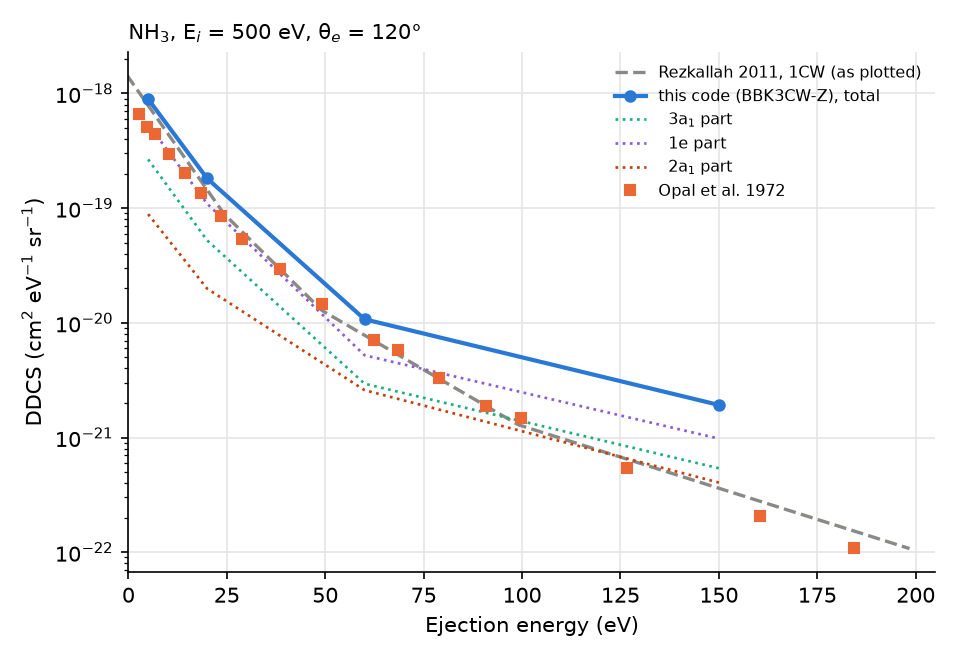
\includegraphics[width=0.62\linewidth]{figs/ddcs.png}
\caption{DDCS of \NH{} at $E_i=500$~eV, $\theta_e=120^\circ$: 3CWZ (total and per orbital), 1CW
of Ref.~\cite{Rezkallah2011}, and experiment~\cite{Opal1972}.}\label{fig:ddcs}
\end{figure}

\subsection{\CH: TDCS}\label{sec:ch4}
\todo{TDCS of the \CH{} 1t$_2$ and 2a$_1$ orbitals with the same code, compared with
Lahmam-Bennani \emph{et al.}~\cite{LahmamBennani2009} (protocol objectives O2, O4). The code
already contains the \CH{} target, so only the kinematics and the orbital switch need setting.}

\subsection{Post-collision interaction}\label{sec:pci}
\todo{Protocol objective O3: results with and without $C_{se}$ (set $C_{se}=1$ and its Gamow
factor to 1) for the \NH{} orbitals at $E_e=74$~eV and for \CH. Discuss the shift of the binary
peak and the change of the recoil-to-binary ratio.}

\subsection{Variable versus constant charge}\label{sec:zconst}
\todo{Expected result 1: the same runs with $Z(r)\equiv1$ for the outgoing electrons and
$Z\equiv0$ for the incident one (3C/BBK limit), to isolate the contribution of the variable
charge.}

%=====================================================================
\section{Discussion: origin of the recoil deficit and domain of validity}\label{sec:discussion}
%=====================================================================
\subsection{The ejected-electron wave}
The recoil peak comes from the ejected electron being back-scattered by the residual ion. Three
results show that the ejected wave of Eq.~(\ref{eq:cwz}) does not contain enough of it.

\textbf{(i) Phase shifts.} We solved the radial equation
$u''+[k^2-l(l+1)/r^2+2Z_{ion}(r)/r]\,u=0$ exactly with the same $Z_{ion}(r)$ at $E_e=74$~eV. The
short-range phase shifts beyond the $Z=1$ Coulomb wave are large
(Table~\ref{tab:delta}). Inside the molecule, the partial waves of the 3CWZ wave keep the $Z=1$
Coulomb phases, and their radial nodes are displaced. The local $\alpha(r)$ in
Eq.~(\ref{eq:cwz}) therefore does not produce a solution of the equation it approximates.

\textbf{(ii) Back-scattering.} The elastic cross section of the electron on NH$_3^+$ obtained with
these phase shifts exceeds the Rutherford ($Z=1$) value by factors 29--137 between $120^\circ$
and $180^\circ$. This is the process the recoil peak requires.

\textbf{(iii) Not a structure effect.} In a plane-wave picture the binary/recoil ratio would be
$\rho(q_{\rm binary})/\rho(q_{\rm recoil})$, with $q\approx1.5$ and $3.2$~a.u.\ here. This gives
38, 59 and 155 for \aone, 1e and \atwo, against 1--2.5 measured. No realistic orbital can account
for the observed recoil.

These findings agree with the failure of the two corrections tested in Section~\ref{sec:results}.
The short-range potential acts mainly through the spurious non-orthogonality. Orthogonalization
removes the spurious part but adds no back-scattering.

\begin{table}[h]\centering\small
\caption{Short-range phase shifts and elastic back-scattering for e$^-$ + NH$_3^+$ at 74 eV.}\label{tab:delta}
\begin{tabular}{lcccccc}\toprule
$l$ & 0 & 1 & 2 & 3 & 4 & 5\\
$\delta_l$ (rad) & 2.60 & 1.34 & 0.48 & 0.26 & 0.17 & 0.09\\\midrule
angle & $30^\circ$ & $60^\circ$ & $90^\circ$ & $120^\circ$ & $150^\circ$ & $180^\circ$\\
$\sigma_{el}/\sigma_{\rm Ruth}(Z=1)$ & 2.5 & 4.8 & 4.9 & 29 & 91 & 137\\\bottomrule
\end{tabular}
\end{table}

\subsection{Domain of validity}
Within the present implementation, the molecular 3CWZ model is reliable for:
\begin{itemize}
\item the position and shape of the binary peak in asymmetric kinematics with small momentum
  transfer;
\item the momentum profiles of EMS, at the level of the PWBA.
\end{itemize}
It is not reliable for:
\begin{itemize}
\item the recoil region and large ejection angles, because of the missing short-range distortion
  of the ejected electron;
\item fast outgoing electrons or large momentum transfer, without grids adapted to $K$.
\end{itemize}
\todo{Revise this section after the \CH, PCI and constant-charge results.}

%=====================================================================
\section{Conclusions and perspectives}\label{sec:conclusion}
%=====================================================================
\textbf{Conclusions.}
\begin{itemize}
\item We extended the 3CWZ model to molecular targets described by Moccia one-centre orbitals.
  The orientation average is analytic, and the effective charges are derived from the Hartree
  potential with a self-interaction correction.
\item We implemented the model in a validated parallel code and applied it to the three valence
  orbitals of \NH.
\item The binary peak is well described.
\item The recoil peak is underestimated by a factor 5--10. We traced this to the ejected-electron
  wave, not to the target description or to the numerics.
\end{itemize}

\textbf{Perspectives.}
\begin{itemize}
\item Replace the ejected 3CWZ wave by the exact distorted wave in the same Hartree potential
  (partial waves up to $l\approx10$, matched to the $Z=1$ Coulomb wave). This keeps the rest of
  the 3CWZ structure, in the spirit of the 1DW calculations for H$_2$O~\cite{Champion2006} and the
  distorted-wave methods~\cite{Madison2010}.
\item Use grids adapted to the momentum transfer, then compute DDCS, SDCS and total cross sections
  (comparison with Ref.~\cite{Rejoub2001}).
\item Include the exchange amplitude and compare with the low-energy data of Nixon
  \emph{et al.}~\cite{Nixon2013}.
\item Extend the model to other molecules of interest (H$_2$O, biomolecular fragments).
\end{itemize}
\todo{Add the conclusions on \CH{} and on the PCI study.}

%=====================================================================
\begin{thebibliography}{99}\small
\bibitem{Brauner1989} M. Brauner, J. S. Briggs, H. Klar, J. Phys. B \textbf{22}, 2265 (1989).
\bibitem{Bechane2024} K. Bechane, S. Houamer, T. Khatir, A. Tamin, C. Dal Cappello, Phys. Rev. A \textbf{109}, 012812 (2024).
\bibitem{Tamin2024} A. Tamin, S. Houamer, T. Khatir, L. U. Ancarani, C. Dal Cappello, J. Chem. Phys. \textbf{161}, 164305 (2024).
\bibitem{Zaidi2024} O. Zaidi, A. Mansouri, S. Houamer, A. Tamin, T. Khatir, C. Dal Cappello, Eur. Phys. J. D \textbf{78}, 140 (2024).
\bibitem{Moccia1964a} R. Moccia, J. Chem. Phys. \textbf{40}, 2164 (1964) [HF, CH$_4$, SiH$_4$].
\bibitem{Moccia1964b} R. Moccia, J. Chem. Phys. \textbf{40}, 2176 (1964) [NH$_3$, NH$_4^+$, PH$_3$, PH$_4^+$].
\bibitem{ElMir2020} R. El Mir, K. Kaja, A. Naja, E. M. Staicu Casagrande, S. Houamer, C. Dal Cappello, J. Phys. B \textbf{54}, 015201 (2021).
\bibitem{Bawagan1988} A. O. Bawagan, R. M\"uller-Fiedler, C. E. Brion, E. R. Davidson, C. Boyle, Chem. Phys. \textbf{120}, 335 (1988).
\bibitem{Opal1972} C. B. Opal, E. C. Beaty, W. K. Peterson, At. Data \textbf{4}, 209 (1972).
\bibitem{Rezkallah2011} Z. Rezkallah, S. Houamer, C. Dal Cappello, I. Charpentier, A. C. Roy, Nucl. Instrum. Methods B \textbf{269}, 2750 (2011).
\bibitem{LahmamBennani2009} A. Lahmam-Bennani, A. Naja, E. M. Staicu Casagrande, N. Okumus, C. Dal Cappello, I. Charpentier, S. Houamer, J. Phys. B \textbf{42}, 165201 (2009).
\bibitem{Nixon2013} K. L. Nixon, A. J. Murray, H. Chaluvadi, C. Ning, J. Colgan, D. H. Madison, J. Chem. Phys. \textbf{138}, 174304 (2013).
\bibitem{Rejoub2001} R. Rejoub, B. G. Lindsay, R. F. Stebbings, J. Chem. Phys. \textbf{115}, 5053 (2001).
\bibitem{Champion2006} C. Champion, C. Dal Cappello, S. Houamer, A. Mansouri, Phys. Rev. A \textbf{73}, 012717 (2006).
\bibitem{Madison2010} D. H. Madison, O. Al-Hagan, J. At. Mol. Opt. Phys. \textbf{2010}, 367180 (2010).
\end{thebibliography}

\end{document}
